\documentclass[conference,onecolumn,11pt]{IEEEtran}
\IEEEoverridecommandlockouts
% The preceding line is only needed to identify funding in the first footnote. If that is unneeded, please comment it out.
\usepackage{amsmath,amssymb,amsfonts}
\usepackage{algorithmic}
\usepackage{graphicx}
\usepackage{textcomp}
\usepackage{xcolor}
\usepackage{hyperref}
\usepackage{booktabs} % for tables
\usepackage[sorting=none]{biblatex}
\addbibresource{cite.bib}


\def\BibTeX{{\rm B\kern-.05em{\sc i\kern-.025em b}\kern-.08em
    T\kern-.1667em\lower.7ex\hbox{E}\kern-.125emX}}
\begin{document}

\title{Predicting Stock Market Volatility with Time Series Models\\
}

\author{\IEEEauthorblockN{1\textsuperscript{st} Xu Hao}
\IEEEauthorblockA{\textit{Department of Mathematics \& Statistics} \\
\textit{Thompson Rivers University}\\
Kamloops, Canada \\
xuh23@mytru.ca}
\and
\IEEEauthorblockN{2\textsuperscript{nd} Mulk Waqar Ul}
\IEEEauthorblockA{\textit{Department of Mathematics \& Statistics} \\
\textit{Thompson Rivers University}\\
Kamloops, Canada \\
mulkw22@mytru.ca}
}

\maketitle

\begin{abstract}
Predicting stock market movements is a significant challenge for traders, investors, and businesses, yet it can be highly profitable with precise forecasts. Achieving accurate predictions is crucial, particularly given the volatile, nonlinear, and unpredictable nature of the stock market. In this paper we are predicting stock prices of Apple using two machine learning algorithms - Linear Regression and Autoregressive Integrated Moving Average (ARIMA) by comparing their forecasting performances. The data is collected from Yahoo Finance and Google Trends and the analysis spans a period of eight years, from April 1st, 2016, to March 31st, 2024. The performance of the models are evaluated by root mean squared error (RMSE), mean squared error (MSE) and R-squared ($R^2$). 
%The findings of this study {\color{red}demonstrate that Simple Linear Regression is not well-suited for time series data analysis, whereas ARIMA presents distinct advantages in forecasting stock prices.}
In this study, we implemented an Autoregressive model with lag-$p$ of predictors using multiple linear regression and compared the results with results from ARIMA $(p,0,0)$. Our conclusion shows that Linear Regression with performs poorly on stock market predictions.

\end{abstract}

\begin{IEEEkeywords}
Forecasting, Stock Prices, Machine Learning, Autoregression, Linear Regression. 
\end{IEEEkeywords}

\section{Introduction}
A stock signifies an investment representing ownership in a company. The total ownership of a company is divided into shares, with each share representing an equal portion of the business. The stock market functions as a marketplace where individuals can purchase shares of stock. 
%Analogous to various other markets like grocery stores or farmers’ markets, where multiple vendors gather to sell their products, the stock market serves as a central hub for trading securities. Similarly to a farmers’ market where different farmers offer their produce, customers have the opportunity to explore various investment options and make purchases according to their preferences. In essence, the stock market operates similarly to these markets, acting as a centralized venue where buyers and sellers converge to trade stocks and other investment instruments, including mutual funds, which pool together multiple stocks. However, unlike a single market, the stock market comprises several smaller markets known as stock exchanges.
Utilizing machine learning algorithms for stock price prediction aids in uncovering the potential future value of company stocks and other financial assets traded on various exchanges.\cite{Vijh2020} The fundamental objective of predicting stock prices is to attain substantial profits. However, forecasting the performance of the stock market is a formidable challenge. Several factors come into play in this prediction process, encompassing both tangible and psychological elements, rational and irrational behaviors, among others.
The interaction of these diverse factors renders share prices highly dynamic and volatile, thereby posing significant hurdles to achieving precise predictions with a high degree of accuracy.


\subsection*{Linear Regression}

Linear regression is a statistical method used to model the relationship between a dependent variable and one or more independent variables by fitting a linear equation to observed data. In essence, it seeks to determine the best-fitting straight line through the data points. The goal is to find the coefficients of the linear equation that minimize the difference between the observed and predicted values of the dependent variable. Linear regression is widely employed for prediction and forecasting tasks, as well as for understanding the relationships between variables in a dataset.

$Y = \beta_0+\beta_1 x_1 + \beta_2 x_2 + \ldots+\beta_n x_p + \epsilon$
$y$ represents the dependent variable, $x_1, x_2, ..., x_p$ represents the independent variables, $\beta_0,\beta_1,\beta_2,\ldots,\beta_p$ represents the coefficients associated with each independent variable, and $p$ is the number of independent variables. $\epsilon$ represents the error term, which captures the difference between the observed and predicted values of the dependent variable.


\subsection*{ARIMA}

ARIMA, or AutoRegressive Integrated Moving Average, is a forecasting algorithm grounded in the principle that historical values of a time series can offer insights into future trends.\cite{Khanderwal2021} Belonging to a class of models renowned for elucidating time series behavior through its own past data, including lags and lagged forecast errors, ARIMA excels in predicting forthcoming values. It is particularly applicable to time series datasets exhibiting discernible patterns rather than random noise. ARIMA entails three key parameters: $p$, $d$, and $q$. The parameter $p$ denotes the number of autoregressive terms or lag observations, providing lagged data points. $d$ signifies the degree of differencing, indicating the number of times lagged indicators have been subtracted to achieve data stationarity. $q$ represents the number of forecast errors in the model, akin to the size of the moving average window. These parameters, integers by nature, are pivotal in defining the ARIMA model's functionality and can take a value of 0, implying their exclusion from the model. ARIMA models are denoted by their parameter combinations, such as ARIMA(1, 0, 0) for the first-order autoregressive model or ARIMA(0, 1, 0) for the random walk model. Consequently, ARIMA can transform into various models: ARMA $(d=0)$, AR $(p>0, d=0, q=0)$, and MA $(p=0, d=0, q>0)$.  Once the parameters are set, the ARIMA model estimates coefficients $\alpha$ and $\theta$, utilizing past data points to forecast future values.

\section{Literature review}

Many researchers have done their studies in predicting stock prices using similar  machine learning models, some of them are discussed below. 

In 2018 \citeauthor{Xu2018} wrote a paper on predicting stock prices for Apple Inc. Her paper focuses on stock price forecasting by combining conventional time series analysis with information from Yahoo Finance and Google Trend. It aims to predict weekly changes in stock price, particularly focusing on Apple Inc. stock. Her study records important news/events related to Apple Inc. over a five-year span and uses the weekly Google trend index values to measure the magnitude of these events. The data includes weekly stock prices of Apple Inc. and key developments from Yahoo Finance, while her analysis involves applying the ARIMA model, differencing the data, and regressing stock price changes on news values. The paper also presents an algorithm for computing the value of news at a certain time, simulating the impact of news on stock prices. Her analysis reveals a significant correlation between the changes in weekly stock prices and the values of important news/events computed from the Google trend website.


\section{Data}
%Waqar's paragraph
%It consists of 6 independent variables and one response variable. The adjusted close price is a variable which we are using both as an independent and dependent variable. %Table 1 shows statistics of the dataset that is used for training and testing.

% \begin{table}[htbp]
%     \centering
%     \caption{Dataset Splitting}
%     \begin{tabular}{@{}rlllll@{}}
%         \toprule
%          && \textbf{Dataset} & \textbf{Training} & \textbf{Validation} & \textbf{Testing} \\
%         \midrule
%         \textbf{Time Interval} &(Start) & 04-01-2016 & 04-01-2016 & 01-02-2021 & 07-01-2023\\
%         &(End)& 03-31-2024 & 01-01-2021 & 06-30-2023 & 03-31-2024\\
  
%         \bottomrule
%     \end{tabular}
%     \label{tab:GFS}
% \end{table}

The stock price data utilized in our analysis is sourced from Yahoo Finance, including daily stock prices and trading volumes across various stocks. Six columns within the dataset serve as potential predictor variables, with five pertaining to stock price metrics (open, close, highest, lowest, and adjusted close prices), and the remaining column representing the volume of each respective stock. We specifically utilize the adjusted close price both as a predictor and response variable. We choose this metric because it is calculated from the other 4 metrics. Additionally, we downloaded Google Trends data reflecting the interest levels over time for five key Apple products, employing these as additional predictor variables. Our analysis is solely focused on Apple stocks, with data spanning from April 1st, 2016, to March 31st, 2024. We merge the data based on the date column. Table~\ref{tab:merged_data} shows the first 6 rows of the merged data.

\begin{table}[ht]
\centering
\begin{tabular}{rrrrrrrrr}
  \hline
 & Date & AdjClosed & Volume & Apple.Watch & MacBook & AirPods & iPad & iPhone \\ 
  \hline
1 & 2016-04-01 & 25.14 & 103496000.00 &   1 &   2 &   0 &   6 &  33 \\ 
  2 & 2016-04-04 & 25.40 & 149424800.00 &   1 &   2 &   0 &   6 &  29 \\ 
  3 & 2016-04-05 & 25.10 & 106314800.00 &   1 &   2 &   0 &   6 &  30 \\ 
  4 & 2016-04-06 & 25.36 & 105616400.00 &   1 &   2 &   0 &   6 &  28 \\ 
  5 & 2016-04-07 & 24.81 & 127207600.00 &   1 &   2 &   0 &   6 &  28 \\ 
  6 & 2016-04-08 & 24.83 & 94326800.00 &   1 &   2 &   0 &   6 &  29 \\ 
   \hline
\end{tabular}
\label{tab:merged_data}
\end{table}

\subsection*{Transformation}

To perform a linear regression on time series data, we first need to make sure the data are independently normally distributed. we need to check the distribution of our response variable which is the adjusted close price of Apple.
The plot of the raw data against the index of the date is shown in Fig.~\ref{fig:price}.

\begin{figure}[htpb]
	\centering
	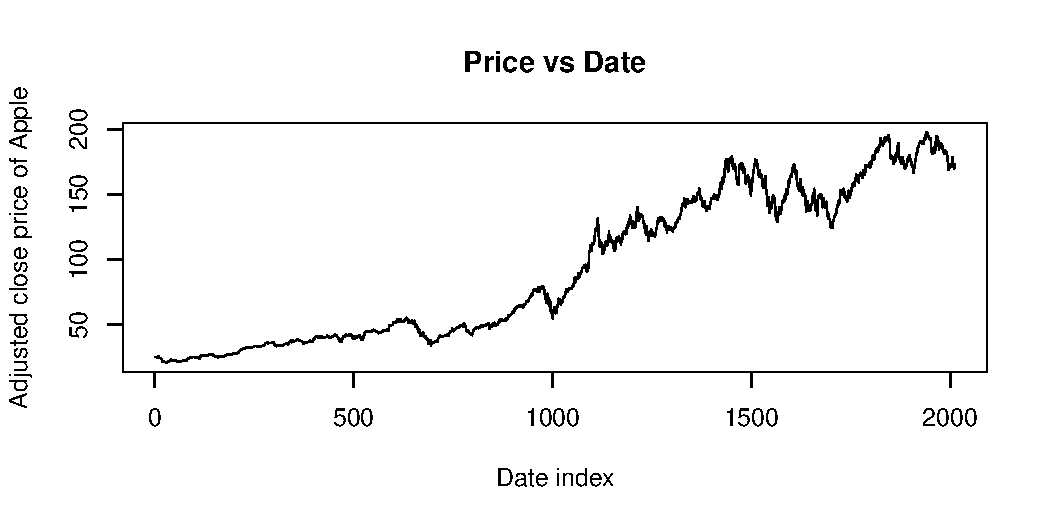
\includegraphics[width=0.8\textwidth]{pic/Price_vs_Date.pdf}
	\caption{}
	\label{fig:price}
\end{figure}

Fig.~\ref{fig:price} shows a increasing trend in the adjusted close price of Apple over the specified eight-year period. However, the movement of the stock price itself doesn't seem to follow a clear pattern. Notably, the variance of the stock price appears to slightly increase over time, with particularly heightened volatility towards the end of the period. These observations suggest that applying a log or square root transformation to the response variable could help stabilize the variance. 

To check for independence, we plotted the autocorrelation of the adjusted close price of Apple in Fig.~\ref{fig:acf1}.

\begin{figure}[htpb]
	\centering
	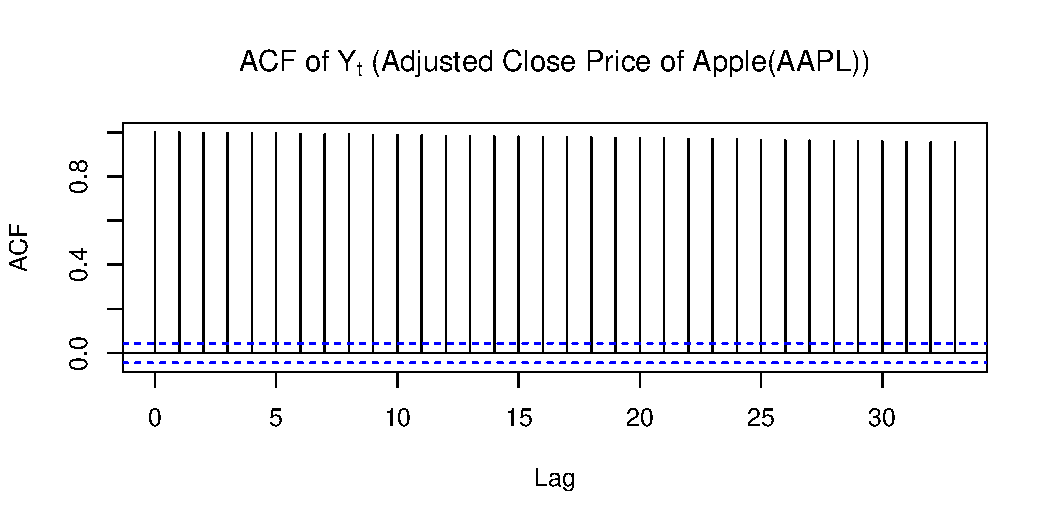
\includegraphics[width=0.8\textwidth]{pic/ACF_AdjClosed.pdf}
	\caption{}
	\label{fig:acf1}
\end{figure}

From Fig.~\ref{fig:acf1} we can see that there is a strong autocorrelation in the adjusted close price of Apple. This suggests that we cannot perform a linear regression directly on the adjusted close price. Instead, we should check for the first difference of the data. The first difference of adjusted close price of Apple in shown in Fig.~\ref{fig:d} and its autocorrelationn is shown in Fig.~\ref{fig:acf2}.

\begin{figure}[htpb]
	\centering
	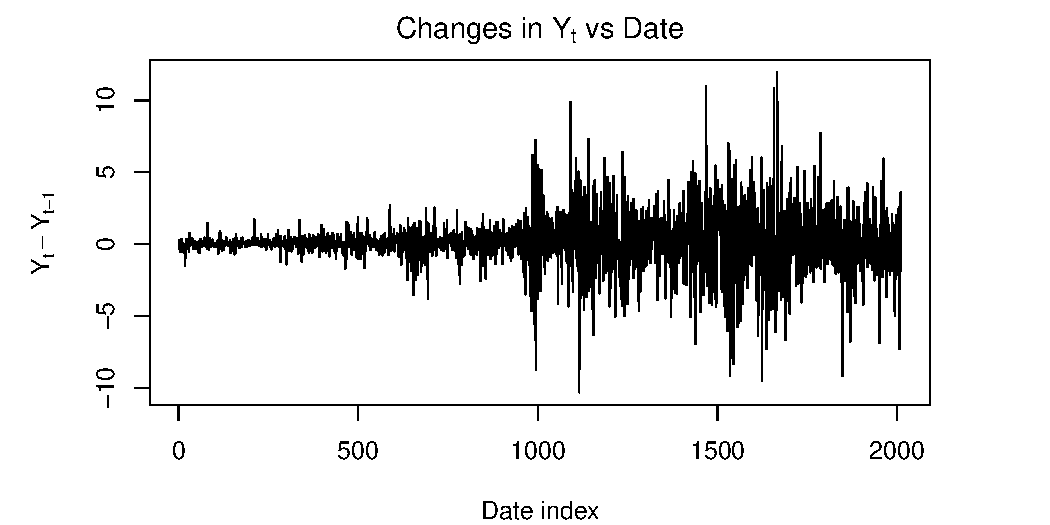
\includegraphics[width=0.8\textwidth]{pic/AdjClosed.pdf}
	\caption{}
	\label{fig:d}
\end{figure}

\begin{figure}[htpb]
	\centering
	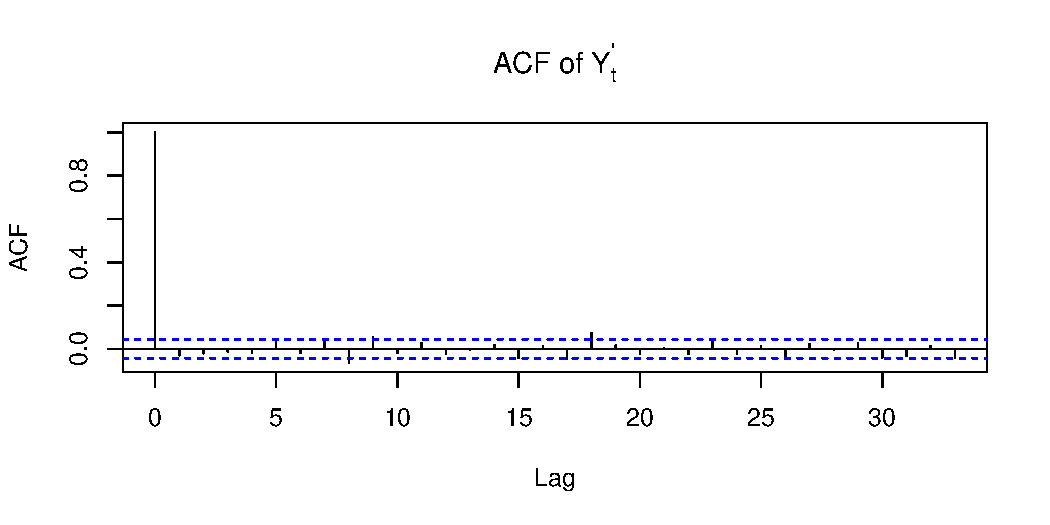
\includegraphics[width=0.8\textwidth]{pic/ACF_dAdjClosed.pdf}
	\caption{}
	\label{fig:acf2}
\end{figure}

From Fig.\ref{fig:acf2} we can see that the autocorrelation problem can be solved by taking the first difference of the response variable. However, in Fig.~\ref{fig:d}, we can see that the variance of the first difference are larger at the end of the time period, which means we have a heteroscedasticity in the response variable. To solve this, we need to take transformation of the response variable. As previously suggested, we are applying a log or square root transformation.

%Plot the graphs of $\sqrt{y_t}-\sqrt{y_{t-1}}$ (as shown in Fig.~\ref{fig:dsqrt}) and $\ln(y_t)-\ln(y_{t-1})$ (as shown in Fig.~\ref{fig:dlog}) to compare.

\begin{figure}[htpb]
	\centering
	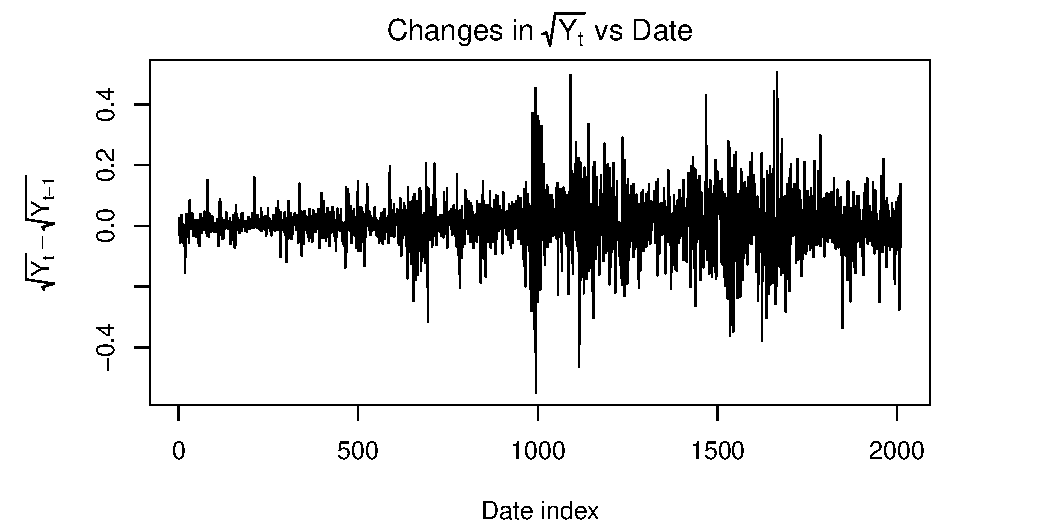
\includegraphics[width=0.8\textwidth]{pic/Sqrt_AdjClosed.pdf}
	\caption{}
	\label{fig:dsqrt}
\end{figure}

\begin{figure}[htpb]
	\centering
	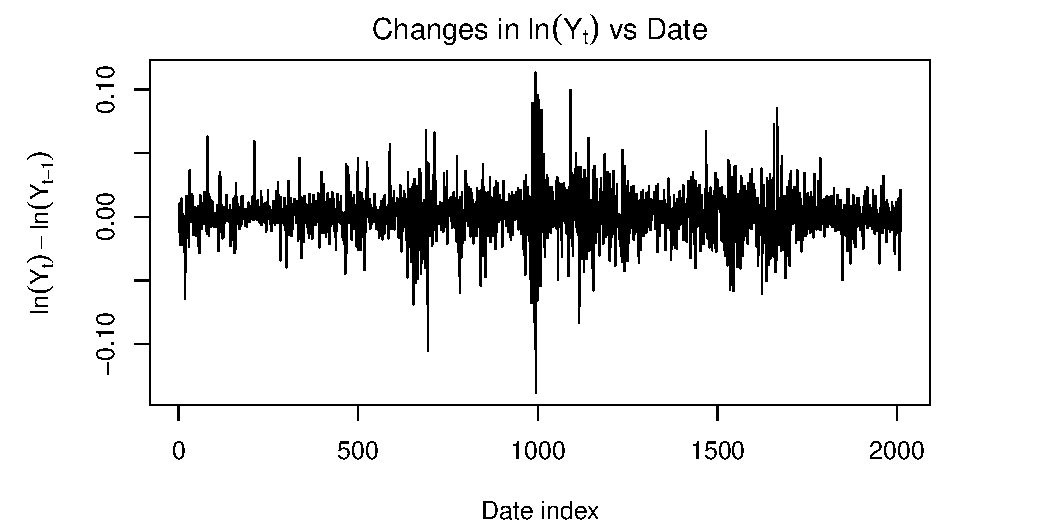
\includegraphics[width=0.8\textwidth]{pic/log_AdjClosed.pdf}
	\caption{}
	\label{fig:dlog}
\end{figure}

Comparing the graphs in Fig.\ref{fig:d}, Fig.\ref{fig:dsqrt} and \ref{fig:dlog}), the variance in the data is more stable in the last two figures. This tells us that transforming the raw data is a good idea. Looking closer at Fig.~\ref{fig:dsqrt} and \ref{fig:dlog}, we see that both the square root and logarithm transformations help to stabilize the variance, and the patterns in the differences look random. We've decided to go with the logarithm transformation because it seems to do the best job of stabilizing the variance.


\section{Method}

\subsection*{Autoregression with one variable}\label{mod1}

We use $y_{t}$ to represent the adjusted close price of Apple stock.
We use $y^{'}_{t} = \ln(y_{t})-\ln(y_{t-1}) = \ln(\frac{y_{t}}{y_{t-1}})$ to represent the first difference of log of $y_{t}$.

We use the autoregression model with Lag-$p$. We defiine our model AR($p$) as follows:

\[
y^{'}_{t} = c + \phi_{1}y^{'}_{t-1} + \phi_{2}y^{'}_{t-2} + \dots + \phi_{p}y^{'}_{t-p} + \varepsilon_{t},
\]

The predicted value for $y_t$ is calculated as follows:

\[
\hat{y}_t = \exp\{c + \phi_{1}y^{'}_{t-1} + \phi_{2}y^{'}_{t-2} + \dots + \phi_{p}y^{'}_{t-p}\}\cdot y_{t-1}
\]

\subsection*{Autoregression with multiple variables}
\label{mod2}

From Google trends, we get the interest over time of keywords ``Apple Watch", ``MacBook", ``AirPods", ``iPad", ``iPhone", represented by variables $y_{3,t},y_{4,t},y_{5,t},y_{6,t},y_{7,t}$ respectively. Also, we take the volume of the apple stock represented by variable $y_{2,t}$, the first difference of the adjusted close price of Apple stock as $y_{1,t}$ (which is also $y^{'}_t$). $\mathbf{y}_t = (y_{1,t},y_{2,t},y_{3,t},y_{4,t},y_{5,t},y_{6,t},y_{7,t})$.

We define our Vector Auto-Regressive(VAR) model as follows:

\[
y^{'}_t = \boldsymbol{\phi}_1\mathbf{y}_{t-1}^T+\ldots+\boldsymbol{\phi}_p\mathbf{y}_{t-p}^T+\epsilon_t
\]

where $\boldsymbol{\phi}_i$ are $(1\times7)$ coefficient vector for $i=1,\ldots,p$.

\subsection*{Implementation}

We implement the autoregression model using the \texttt{lm} function in R.\footnote{The source code is provided here: \url{https://github.com/cld4h/DASC5420_Project}} When only using the adjusted close price as the predictor variables, we compare the result from \texttt{lm} with the result from \texttt{arima(data, order=c(p,0,0))}. For example, the fitted model of \texttt{AR(3)} is shown in Table~\ref{tab:regression}. The pairwise scatterplot of the predictor and response variables is shown in Fig.~\ref{fig:pairwise}.

\begin{table}[htbp]
  \centering
  \caption{Regression Coefficients}
  \begin{tabular}{lcc}
    \toprule
    \textbf{Variable} & \textbf{Coefficient from \texttt{lm}} & \textbf{Coefficient from \texttt{arima(data, order=c(p,0,0))}}\\
    \midrule
    Intercept & 0.0010389 & 1e-3\\
    $y^{'}_{t-1}$ & -0.0758287 & ar1=-0.0761\\
    $y^{'}_{t-2}$ & 0.0005033 & ar2=0.0006\\
    $y^{'}_{t-3}$ & -0.0152322 & ar3=-0.0152\\
    \bottomrule
  \end{tabular}
  \label{tab:regression}
\end{table}

\begin{figure}[htpb]
	\centering
	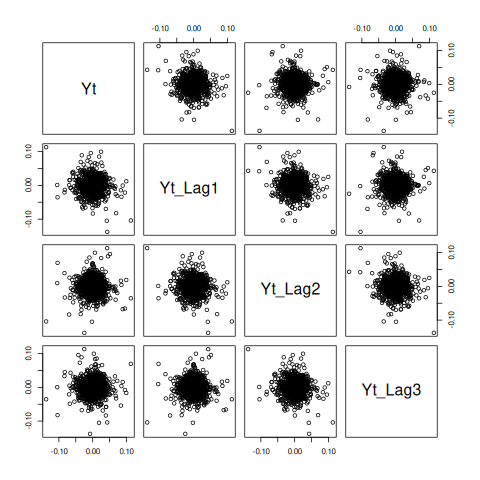
\includegraphics[width=0.4\textwidth]{pic/pairwise.png}
	\caption{Pairwase scatterplot of $y^{'}_t$ and its lagged features}
	\label{fig:pairwise}
\end{figure}

From Fig.~\ref{fig:pairwise} we see that there is no linear relationship between $y^{'}_t$ and its lagged values. This tells us that we need to include additional information like Google Trends key words to improve the model performance.

Performing Autoregression on $\mathbf{y}_t = (y_{1,t},y_{2,t},y_{3,t},y_{4,t},y_{5,t},y_{6,t},y_{7,t})$ with a Lag of $p$ will give us $7\times p$ predictor variables. This makes our model complecated. In this case, we need to perform a variable selection. 

Here we are usign stepwise regression employing the Akaike Information Criterion (AIC). This method iteratively selects the most relevant predictors to include in a regression model, aiming to maximize explanatory power while minimizing complexity. By considering the AIC, which balances model fit and parsimony, stepwise regression helps identify the optimal subset of predictors, thereby enhancing the interpretability and predictive accuracy of the model. In the context of time series analysis, where data points are chronologically ordered, stepwise regression with AIC serves as a valuable tool for uncovering meaningful relationships and understanding the underlying dynamics driving the observed temporal patterns.


\section{Results}

In this project, we select a $p=10$ as our lagged values and perform a 5-folds cross validation on the first 1900 data. We use the last 100 data to test our model performance. The predicted value of  $y^{'}_t$ and $y_t$ are plotted in Fig.\ref{fig:pred_dprice} and \ref{fig:pred_price} respectively.

\begin{figure}[htpb]
	\centering
	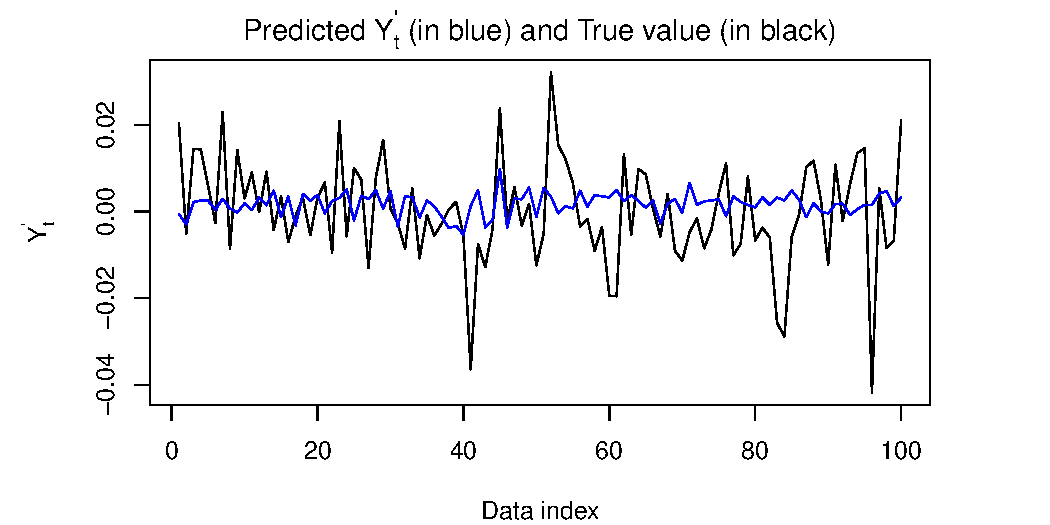
\includegraphics[width=0.8\textwidth]{pic/Predicted_dAdjColsed.pdf}
	\caption{The predicted first log difference}
	\label{fig:pred_dprice}
\end{figure}

\begin{figure}[htpb]
	\centering
	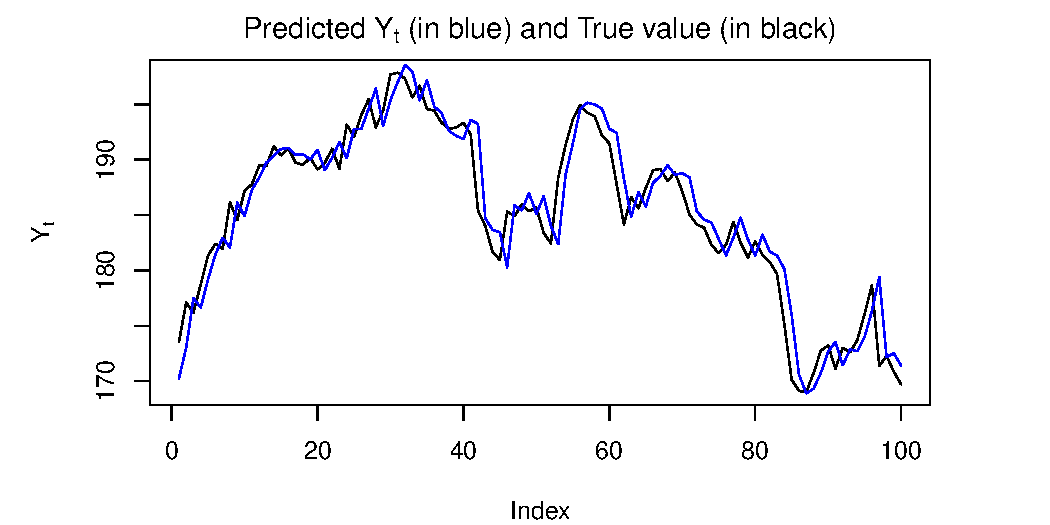
\includegraphics[width=0.8\textwidth]{pic/Predicted_AdjColsed.pdf}
	\caption{The predicted adjusted close price}
	\label{fig:pred_price}
\end{figure}

\section{Discussion and Conclusion}

From Fig.~\ref{fig:pred_price} we can see our model performance is not good. The prediction is very close to the adjusted close price one day earlier. This can be explained by Fig.~\ref{fig:pred_dprice}: the value of predicted $y^{'}_t$ is very close to 0. Since the predicted value is calculated by $y_{t-1}\times e^{y^{'}_{t}}$ where $e^{y^{'}_{t}}$ is close to $1$ when $y^{'}_t\approx0$.

In conclusion, the linear regression model gives a bad performance at predicting the apple stock market data using Google Trends keywords of apple products. One can try some more advance models like LSTM and incorporate some additional predictor variables to improve the performance\cite{Aasi2021}.

\printbibliography

\vspace{12pt}
\end{document}
